\documentclass[nooutcomes]{ximera}
%\documentclass[space,handout,nooutcomes]{ximera}

% For preamble materials

\usepackage{pgf,tikz}
\usepackage{mathrsfs}
\usetikzlibrary{arrows}
\usepackage{framed}
\usepackage{amsmath}
\pgfplotsset{compat=1.17}

\def\fixnote#1{\begin{framed}{\textcolor{red}{Fix note: #1}}\end{framed}}  % Allows insertion of red notes about needed edits
%\def\fixnote#1{}

\def\detail#1{{\textcolor{blue}{Detail: #1}}}   

\pdfOnly{\renewenvironment{image}[1][]{\begin{center}}{\end{center}}}

\graphicspath{
  {./}
  {chapter1/}
  {chapter2/}
  {chapter4/}
  {proofs/}
  {graphics/}
  {../graphics/}
}

\newenvironment{sectionOutcomes}{}{}


%%% This set of code is all of our user defined commands
\newcommand{\bysame}{\mbox{\rule{3em}{.4pt}}\,}
\newcommand{\N}{\mathbb N}
\newcommand{\C}{\mathbb C}
\newcommand{\W}{\mathbb W}
\newcommand{\Z}{\mathbb Z}
\newcommand{\Q}{\mathbb Q}
\newcommand{\R}{\mathbb R}
\newcommand{\A}{\mathbb A}
\newcommand{\D}{\mathcal D}
\newcommand{\F}{\mathcal F}
\newcommand{\ph}{\varphi}
\newcommand{\ep}{\varepsilon}
\newcommand{\aph}{\alpha}
\newcommand{\QM}{\begin{center}{\huge\textbf{?}}\end{center}}

\renewcommand{\le}{\leqslant}
\renewcommand{\ge}{\geqslant}
\renewcommand{\a}{\wedge}
\renewcommand{\v}{\vee}
\renewcommand{\l}{\ell}
\newcommand{\mat}{\mathsf}
\renewcommand{\vec}{\mathbf}
\renewcommand{\subset}{\subseteq}
\renewcommand{\supset}{\supseteq}
%\renewcommand{\emptyset}{\varnothing}
%\newcommand{\xto}{\xrightarrow}
%\renewcommand{\qedsymbol}{$\blacksquare$}
%\newcommand{\bibname}{References and Further Reading}
%\renewcommand{\bar}{\protect\overline}
%\renewcommand{\hat}{\protect\widehat}
%\renewcommand{\tilde}{\widetilde}
%\newcommand{\tri}{\triangle}
%\newcommand{\minipad}{\vspace{1ex}}
%\newcommand{\leftexp}[2]{{\vphantom{#2}}^{#1}{#2}}

%% More user defined commands
\renewcommand{\epsilon}{\varepsilon}
\renewcommand{\theta}{\vartheta} %% only for kmath
\renewcommand{\l}{\ell}
\renewcommand{\d}{\, d}
\newcommand{\ddx}{\frac{d}{dx}}
\newcommand{\dydx}{\frac{dy}{dx}}


\usepackage{bigstrut}


\title{Similar Right Triangles}
\author{Brad Findell}
\begin{document}
\begin{abstract}
Proofs. 
\end{abstract}
\maketitle


\begin{problem}
Adapted from Ohio's 2017 Geometry released item 17. 

\begin{image}
\definecolor{qqwuqq}{rgb}{0.,0.39215,0.}
\definecolor{uuuuuu}{rgb}{0.2667,0.2667,0.2667}
\definecolor{qqqqff}{rgb}{0.,0.,1.}
\begin{tikzpicture}[line cap=round,line join=round,>=triangle 45,x=1.0cm,y=1.0cm]
%\clip(-0.75,-1) rectangle (2.9,3.5);
\clip(-2,-1) rectangle (4,3.5);
\draw[line width=0.8pt,color=qqwuqq,fill=qqwuqq,fill opacity=0.1] (0.,0.) -- (0.,0.25) -- (0.25,0.25) -- (0.25,0.) -- cycle; 
\draw[line width=0.8pt,color=qqwuqq,fill=qqwuqq,fill opacity=0.1] (1.2457,1.1314) -- (1.0373,0.9925) -- (1.1762,0.7842) -- (1.3846,0.9231) -- cycle; 
\draw[line width=0.8pt,color=qqwuqq,fill=qqwuqq,fill opacity=0.1] (1.1762,0.7842) -- (1.3152,0.5758) -- (1.5235,0.7147) -- (1.3846,0.9231) -- cycle; 
\draw [line width=0.8pt] (0.,0.)-- (2.,0.);
\draw [line width=0.8pt] (0.,3.)-- (0.,0.);
\draw [line width=0.8pt] (0.,3.)-- (2.,0.);
\draw [line width=0.8pt,dash pattern=on 3pt off 3pt] (0.,0.)-- (1.3846,0.9231);
\begin{scriptsize}
\draw [fill=qqqqff] (0.,0.) circle (1.2pt);
\draw[color=qqqqff] (-0.3154,0.2231) node {$A$};
\draw [fill=qqqqff] (2.,0.) circle (1.2pt);
\draw[color=qqqqff] (2.2108,0.2467) node {$B$};
\draw [fill=qqqqff] (0.,3.) circle (1.2pt);
\draw[color=qqqqff] (0.2276,3.2215) node {$C$};
\draw [fill=uuuuuu] (1.3846,0.9231) circle (1.2pt);
\draw[color=uuuuuu] (1.5497,1.2619) node {$D$};
\end{scriptsize}
\end{tikzpicture}
\end{image}

%\begin{image}
%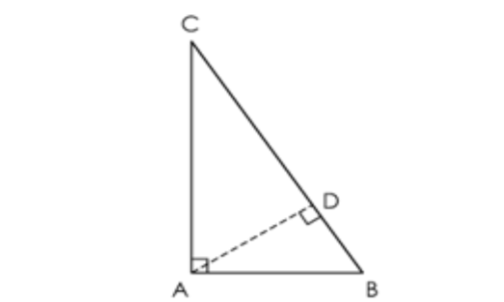
\includegraphics{Q17.png}
%\end{image}
Complete the following proof that $\triangle DAC$ is similar to $\triangle DBA$: 

\begin{enumerate}
\item $\triangle ABC\sim \triangle \answer[format=string]{DBA}$ by AA because they share $\angle B$ and they each have a right angle. 

\item $\triangle ABC\sim \triangle \answer[format=string]{DAC}$ by AA because they share $\angle C$ and they each have a right angle. 

\item $\triangle DAC\sim \triangle \answer[format=string]{DBA}$ because they are both similar to
$\triangle ABC$.
\end{enumerate}
\end{problem}


\end{document}
